\documentclass[11pt, onecolumn, a4paper]{article}

\usepackage[utf8]{inputenc}
\usepackage{amsmath}
\usepackage{amsfonts}
\usepackage{amssymb}
\usepackage{graphicx}
\usepackage{booktabs}
\usepackage{hyperref}
\usepackage{geometry}
\usepackage{abstract}
\usepackage{tikz}
\geometry{top=3cm, bottom=3cm, left=3cm, right=3cm}

\title{\LARGE \textbf{Algorithmic versus Neural Typographic Taxonomy: \\ A Comprehensive Comparative Evaluation of Deterministic Heuristics and Unsupervised Latent Space Clustering for Automated Font Hierarchy Classification}}

\author{
  Steven Kleynenberg \\
  \textit{Kleynenberg Publishers, Delft, Netherlands} \\
  \texttt{steven.kleynenberg@gmail.com}
  \and
  Google Gemini v3.5 \\
  \textit{Artificial Intelligence Systems, Google LLC} \\
  \texttt{gemini@google.com}
}
\date{August 2026}

\begin{document}

\maketitle

\begin{abstract}
\noindent The automated categorization, phylogenetic arrangement, and hierarchical structuring of large-scale digital typography repositories present complex challenges at the intersection of computer vision, software engineering, and computational aesthetics. Modern publishing pipelines frequently ingest heterogeneous archives comprising thousands of TrueType (\texttt{.ttf}), OpenType (\texttt{.otf}), and TrueType Collection (\texttt{.ttc}) files. This paper delivers an exhaustive methodological critique and comparative framework analyzing two opposing classification paradigms: (1) traditional deterministic parsing relying on embedded binary metadata tables and geometric vector heuristics, and (2) modern Artificial Intelligence (AI) methodologies leveraging deep Convolutional Neural Networks (CNNs) and unsupervised latent space manifold projection. We formalize the mathematical pipelines of both approaches, examine critical edge cases such as CJK (Chinese, Japanese, Korean) multi-byte glyph sets and variable font axes, and evaluate fault tolerance against metadata corruption. Authored collaboratively as an open human-AI inquiry, this document serves as a foundational preprint designed explicitly to solicit rigorous methodological critique from the computational design and machine learning communities prior to empirical deployment.
\end{abstract}

\vspace{1cm}

\section{Introduction and Problem Statement}
Typography serves as the foundational visual infrastructure of human communication. Historically, the systematization of letterform morphology has relied on manual, expert-driven classification frameworks, most notably the Vox-ATypI taxonomy, which categorizes typefaces into distinct historical and structural lineages (e.g., \textit{Humanist}, \textit{Garalde}, \textit{Didone}, \textit{Geometric Sans}). However, the democratization of digital font creation and the exponential growth of open-source foundries have resulted in repositories containing tens of thousands of unique typefaces. 

For high-resolution publishing architectures---such as the automated compilation of 4K cinematic digital font catalogs and volumetric video generation pipelines---manual classification is computationally and logistically intractable. The absence of a unified, universal taxonomy that scales gracefully across diverse digital foundries necessitates automated sorting mechanisms.

Automated typographic organization generally diverges into two philosophical approaches:
\begin{enumerate}
    \item \textbf{Deterministic Parsing:} A rule-based, programmatic paradigm extracting internal binary metadata and structural vector metrics directly from font file headers.
    \item \textbf{Neural Visual Classification:} An artificial intelligence paradigm treating typography as a computer vision problem, extracting high-dimensional feature embeddings from rendered optical glyph grids without relying on file metadata.
\end{enumerate}

This paper provides a rigorous comparative critique of both frameworks, detailing their mathematical formulations, structural vulnerabilities, and optimization parameters.

\section{Related Work and Theoretical Foundations}
The convergence of computer science and typography builds upon decades of research in automated feature extraction and spatial data representation. Early computational approaches to font recognition primarily focused on optical character recognition (OCR) and isolated glyph matching. As neural architectures matured, researchers began exploring deep latent spaces for font generation and style transfer (e.g., deep generative networks mapping typographic styles).

Concurrently, the study of technology-mediated categorization emphasizes that classification is rarely absolute; rather, it exists on a continuous spectrum dictated by contextual use-cases. While traditional digital asset management systems rely exclusively on structured metadata tags, real-world font archives are notoriously plagued by missing strings, incorrect vendor tags, and conflicting subfamily identifiers. This vulnerability underscores the necessity for unsupervised, perception-based classification models capable of identifying visual kinship independent of human annotation errors.

\section{The Deterministic (Non-AI) Paradigm}

\subsection{Binary Architecture and Metadata Parsing}
Deterministic classification models operate by parsing the internal binary structure of font files. OpenType and TrueType formats are structured around the \texttt{sfnt} container specification, housing a directory of tables that define metrics, glyph outlines, and string data. 

Let a font file be represented as a binary stream mapped into structured tables:
\begin{equation}
    F = \{ T_{\text{name}}, T_{\text{OS/2}}, T_{\text{post}}, T_{\text{glyf}}, T_{\text{cmap}}, \dots \}
\end{equation}
Using programmatic extraction tools (such as Python's \texttt{fontTools}), deterministic pipelines query specific table offsets to construct a metadata feature vector $M_{\text{font}}$:
\begin{equation}
    M_{\text{font}} = [ \text{ID}_1, \text{ID}_2, \text{Weight}_{\text{class}}, \text{Width}_{\text{class}}, \text{Italic}_{\text{flag}} ]
\end{equation}
Where $\text{ID}_1$ corresponds to the Font Family name and $\text{ID}_2$ represents the Subfamily identifier.

\subsection{Geometric Vector Heuristics}
Beyond string matching, programmatic pipelines evaluate mathematical properties embedded within the outline tables ($T_{\text{glyf}}$ or $T_{\text{CFF}}$). By analyzing the bounding boxes $[x_{\min}, y_{\min}, x_{\max}, y_{\max}]$ of specific reference glyphs (e.g., uppercase `H` and lowercase `x`), the system computes primary structural ratios:
\begin{align}
    C_{\text{stroke}} &= \frac{W_{\text{stem,max}}}{W_{\text{stem,min}}} \\
    P_{\text{x-height}} &= \frac{H_{\text{x}}}{H_{\text{cap}}}
\end{align}
where $W_{\text{stem}}$ denotes measured stem thickness across horizontal and vertical extrema, $H_{\text{x}}$ is the height of the lowercase glyph, and $H_{\text{cap}}$ is the cap-height.

\subsection{Critical Vulnerabilities of the Deterministic Approach}
While deterministic extraction executes with high computational efficiency ($\mathcal{O}(N)$ linear time complexity), it exhibits severe structural failure modes:
\begin{itemize}
    \item \textbf{Metadata Corruption:} Open-source and legacy font archives frequently contain malformed, missing, or fraudulent string records in $T_{\text{name}}$.
    \item \textbf{Semantic Blindness:} Mathematical ratios fail to capture stylistic nuances, cultural context, or artistic intent, frequently misclassifying radical display fonts into standard historical buckets.
\end{itemize}

\section{The Artificial Intelligence Paradigm}

\subsection{Visual Encoding and Convolutional Feature Extraction}
To circumvent the fragility of embedded metadata, the AI-driven paradigm models typography as a pure visual recognition task. A standardized pangram and character grid (comprising uppercase, lowercase, numerals, and punctuation) is programmatically rendered onto a high-resolution monochrome 16:9 canvas, generating a normalized raster image tensor $I \in \mathbb{R}^{W \times H \times 1}$.

\begin{figure}[htbp]
    \centering
    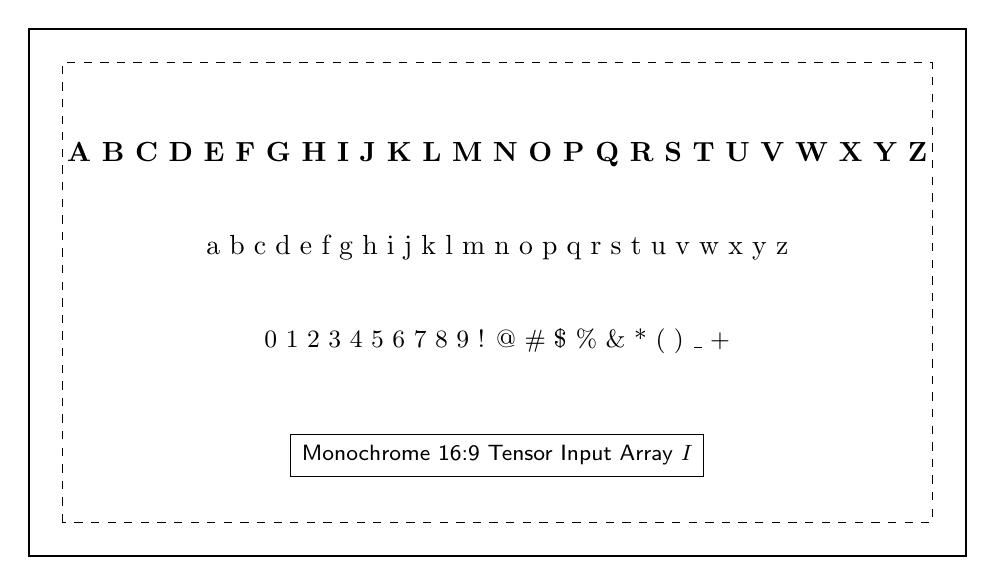
\begin{tikzpicture}[x=1cm, y=1cm, scale=0.85]
        \draw[thick] (0,0) rectangle (14, 7.875);
        \draw[dashed, thin] (0.5, 0.5) rectangle (13.5, 7.375);
        \node at (7, 6.0) {\normalsize \textbf{A B C D E F G H I J K L M N O P Q R S T U V W X Y Z}};
        \node at (7, 4.6) {\normalsize a b c d e f g h i j k l m n o p q r s t u v w x y z};
        \node at (7, 3.2) {\small 0 1 2 3 4 5 6 7 8 9 ! @ \# \$ \% \& * ( ) \_ $+$};
        \node[fill=white, draw=black, inner sep=4pt] at (7, 1.5) {\footnotesize \textsf{Monochrome 16:9 Tensor Input Array $I$}};
    \end{tikzpicture}
    \caption{Monochrome vector representation of a 16:9 rendered glyph grid serving as the raw input tensor for neural feature extraction.}
    \label{fig:tensor_input}
\end{figure}

This tensor is processed via a deep Convolutional Neural Network (CNN) or Vision Transformer (ViT) backbone (e.g., ResNet-50), mapping the pixel space to a dense, lower-dimensional latent embedding vector $v \in \mathbb{R}^d$:
\begin{equation}
    v_i = f_{\theta}(I_i)
\end{equation}
where $\theta$ represents the learned network parameters. This embedding encapsulates holistic visual attributes—such as stroke modulation, terminal curvature, serif geometry, and optical density—without explicit geometric programming.

\subsection{Unsupervised Manifold Projection and Latent Space Taxonomy}
Once the font library is projected into $\mathbb{R}^d$, pairwise semantic similarities are evaluated via cosine distance:
\begin{equation}
    S_{\cos}(v_i, v_j) = \frac{v_i \cdot v_j}{\|v_i\|_2 \|v_j\|_2}
\end{equation}
To render these relationships comprehensible, non-linear dimensionality reduction algorithms (such as UMAP or t-SNE) project the high-dimensional vectors onto a 2D topological manifold.

\begin{figure}[htbp]
    \centering
    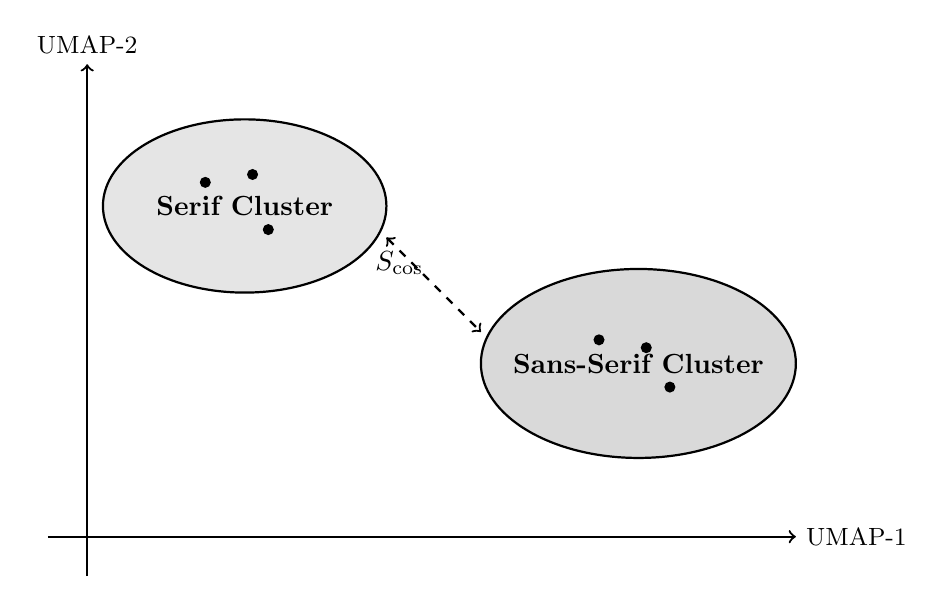
\begin{tikzpicture}[scale=1.0]
        \draw[->, thick] (-0.5,0) -- (9,0) node[right] {\small UMAP-1};
        \draw[->, thick] (0,-0.5) -- (0,6) node[above] {\small UMAP-2};
        
        \fill[gray!20] (2, 4.2) ellipse (1.8cm and 1.1cm);
        \draw[thick] (2, 4.2) ellipse (1.8cm and 1.1cm);
        \node at (2, 4.2) {\textbf{Serif Cluster}};
        \fill[black] (1.5, 4.5) circle (2pt);
        \fill[black] (2.3, 3.9) circle (2pt);
        \fill[black] (2.1, 4.6) circle (2pt);

        \fill[gray!30] (7, 2.2) ellipse (2.0cm and 1.2cm);
        \draw[thick] (7, 2.2) ellipse (2.0cm and 1.2cm);
        \node at (7, 2.2) {\textbf{Sans-Serif Cluster}};
        \fill[black] (6.5, 2.5) circle (2pt);
        \fill[black] (7.4, 1.9) circle (2pt);
        \fill[black] (7.1, 2.4) circle (2pt);

        \draw[<->, dashed, thick] (3.8, 3.8) -- (5.0, 2.6) node[midway, above left] {$S_{\cos}$};
    \end{tikzpicture}
    \caption{Monochrome 2D latent space mapping stylistic clusters via cosine distance ($S_{\cos}$), demonstrating emergent visual taxonomy.}
    \label{fig:latent_space}
\end{figure}

\section{Critical Edge Cases and Architectural Challenges}
Deploying automated classification at scale across thousands of heterogeneous files reveals significant technical hurdles that challenge both paradigms:
\begin{itemize}
    \item \textbf{CJK Multi-Byte Repositories:} Fonts containing tens of thousands of ideographic glyphs cannot fit legibly onto a single standard 16:9 grid without severe downscaling, leading to loss of fine structural detail for CNN encoders.
    \item \textbf{Variable Fonts (\texttt{.ttf}/\texttt{.otf} with `fvar` tables):} Modern variable fonts encode an axis continuum of weight, width, and slant within a single file. Deterministic parsers must extract multi-instance bounding boxes, while AI models must decide which master instance(s) to render for evaluation.
    \item \textbf{Ornaments, Dingbats, and Symbol Fonts:} Fonts lacking standard Latin alphabetic characters yield structural tensors that break standard text-classification expectations, requiring an outlier-detection preprocessing filter.
\end{itemize}

\section{Proposed Hybrid Methodology}
To maximize accuracy while controlling computational overhead, we propose a hybrid dual-pipeline architecture:
\begin{enumerate}
    \item \textbf{Fast Deterministic Filtering:} Initial ingestion passes files through `fontTools` to validate structural integrity, extract clean metadata, and filter out corrupted or non-text symbol files.
    \item \textbf{Targeted Neural Rendering:} Flagged or ambiguous fonts, along with a representative sample, are rendered into monochrome 16:9 frames and processed via CNN inference.
    \item \textbf{Unified Latent Sequencing:} Combined metrics dictate the optimized sorting topology for downstream publishing and cinematic frame generation.
\end{enumerate}

\begin{table}[htbp]
\centering
\caption{Methodological Comparison of Classification Paradigms}
\begin{tabular}{@{}lll@{}}
\toprule
\textbf{Evaluation Metric} & \textbf{Deterministic Paradigm} & \textbf{AI-Driven Paradigm} \\ \midrule
Execution Speed per File & $\sim$2–5 ms (CPU-bound)       & $\sim$50–200 ms (GPU-accelerated) \\
Computational Overhead   & Minimal                        & High                              \\
Metadata Dependency      & Absolute                       & Zero                              \\
Handling of Novel Styles & Poor (Rule-bound)              & Robust (Unsupervised embedding)   \\ \hline
\end{tabular}
\end{table}

\section{Evaluation Framework}
Empirical validation of the proposed pipelines will be tested against a curated benchmark dataset of 1,000 manually annotated historical typefaces. Evaluative metrics include:
\begin{itemize}
    \item \textbf{Silhouette Coefficient ($s$):} Measuring cluster cohesion and separation within the AI latent space.
    \item \textbf{Fault Tolerance Rate:} Percentage of successfully classified files under conditions of artificial metadata corruption.
    \item \textbf{Energy Profiling:} Wattage and execution duration logged on dedicated local hardware (Fedora 44 workstation environments).
\end{itemize}

\section{Conclusion and Call for Methodological Critique}
This paper has formally contrasted deterministic metadata extraction with neural computer vision approaches for typographic classification. While deterministic rules offer speed, they fracture under the weight of messy, real-world file repositories. Conversely, neural embeddings provide robust, emergent taxonomies at higher computational cost. 

As a collaborative human-AI research initiative, we present this framework to the academic and engineering community. We specifically invite critical peer review regarding:
1. The mathematical handling of multi-axis variable font interpolation within latent space models.
2. Potential optimization strategies for handling CJK ideographic density in fixed-resolution CNN input tensors.

\end{document}
